\documentclass[12pt]{article}
\usepackage{url, hyperref, geometry, amsmath, amsfonts, amsthm, nicefrac, graphicx}
\usepackage[table,xcdraw]{xcolor}

\geometry{paper=letterpaper, textheight=9.0in, textwidth=6.5in}

\hypersetup{ 
pdftitle = {Artificial Intelligence 600.335, Spring 2015, Homework 1},
pdfauthor = {Corbin Rosset}
}

\newcommand{\ttt}[1]{\texttt{#1}}
\newcommand{\n}{\vspace{5mm}}

\newenvironment{questionList}{
\newcounter{ctr}
\begin{list}{\textbf{Question \arabic{ctr}.} \\ \\ }
  {\usecounter{ctr}}
  }{
\end{list}
}



\title{Homework 1: Search\\ \normalsize\emph{Artificial Intelligence 600.335, Spring 2015}}
\date{\emph{due date:} February 13th, 2009}
\author{Corbin Rosset}

\begin{document}
\maketitle

\begin{abstract}
  For this assignment, students implemented search algorithms including
  Breadth First Search, Depth First Search, and A* Search.  They applied
  these algorithms to a variety of problems to examine the strengths and
  weaknesses of each algorithm.  Then they answered a set of questions about
  their observations, including both practical and theoretical analysis of the
  algorithms involved.
\end{abstract}

\section{Written Questions}





Consider the following search problem.  A robot is in the living room,
when its owner asks it to go and get him a beer so he won't miss any of the
riveting commercials that are on TV.  The program controlling the robot knows
some information about the layout of the house, and how to get from location to
location, but needs to plan a path that will take it from its current location
in the living room to the kitchen (where the fridge with the beer is).

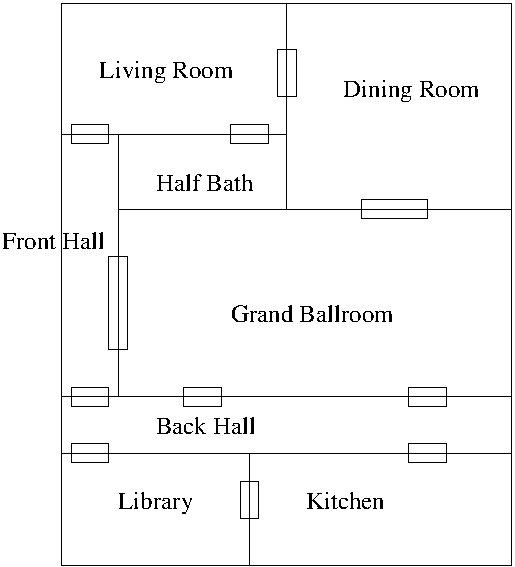
\includegraphics[scale=0.85]{./images/house.pdf}
\n

The agent has the following map of the house, and knows how to move between
rooms. The costs for moving between each pair of rooms with a door connecting
them are listed in the following table.  The costs are the same for the reverse
directions (ie. the cost of going from A to B is the same as the cost of going
from B to A), so only one direction is specified.

\n
\begin{tabular}{|l|l|l|}
  \hline
  & & Cost \\
  \hline
  Living Room & Dining Room & 1 \\
  \hline
  Living Room & Front Hall & 2 \\
  \hline
  Living Room & Half Bath & 1 \\
  \hline
  Front Hall & Back Hall & 1 \\
  \hline
  Front Hall & Grand Ballroom & 3 \\
  \hline
  Dining Room & Grand Ballroom & 2 \\
  \hline
  Back Hall & Grand Ballroom & 2 \\
  \hline
  Back Hall & Library & 1 \\
  \hline
  Back Hall & Kitchen & 2 \\
  \hline
  Library & Kitchen & 2 \\
  \hline
\end{tabular}
\n

The relevant state consists of what room the agent is currently in.  The start
state is the agent being in the library, and the goal is the agent being in the
kitchen.  The actions available to the agent and their costs are defined by the
above table.

\begin{questionList}
\item
Draw a graph of the state-space for this search problem.  Be sure to include and
label all nodes with appropriate names and all edges with the correct weights.

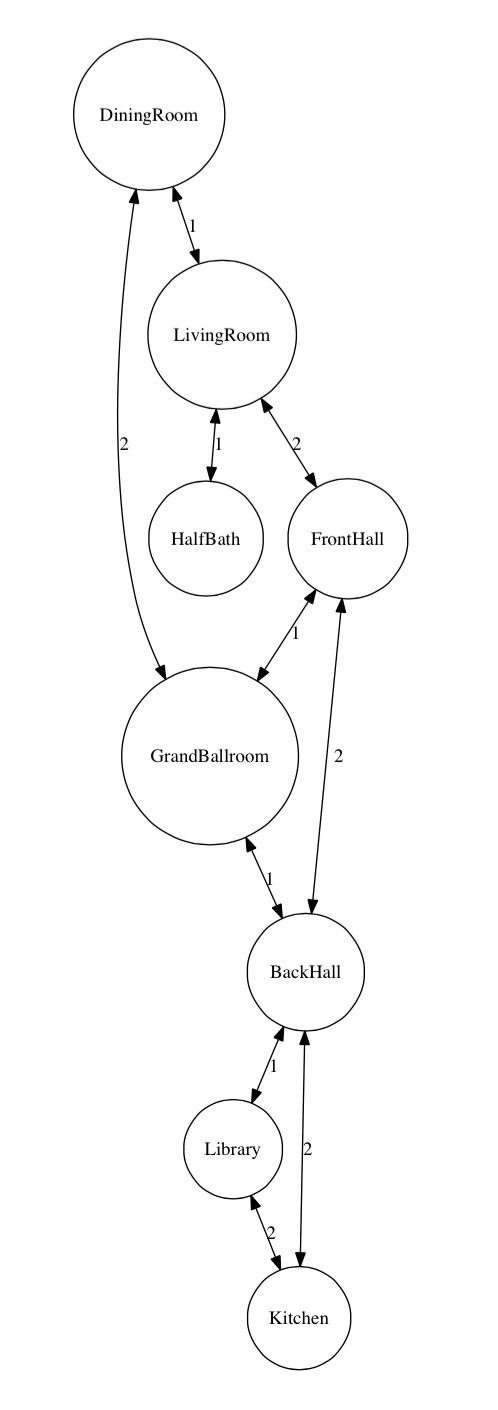
\includegraphics[scale=1]{./images/HouseStateSpace.png}

\item
Draw a graph of the search tree that will be created if the agent uses the
Depth First Seach strategy to solve this problem.  

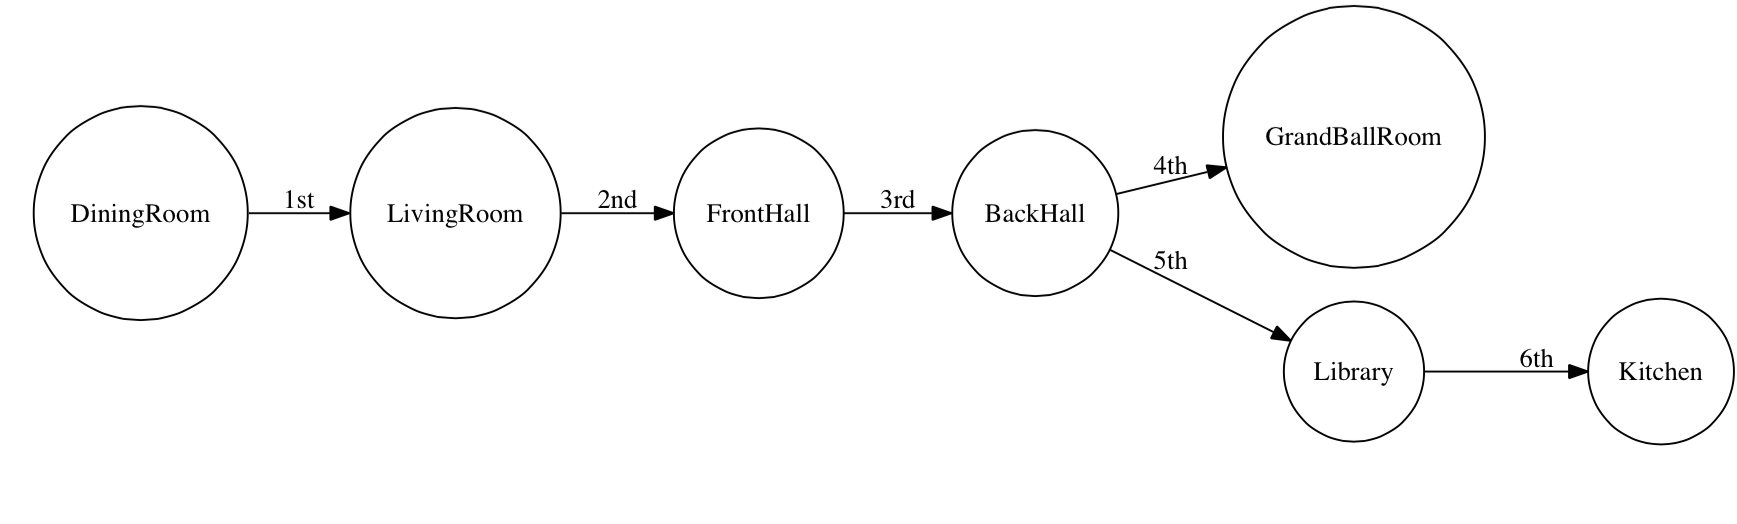
\includegraphics[scale=.5]{./images/DFS.png}

The total cost of the path to the Kitchen is 8. 

Here I am assuming that the robot stands in the middle of the room, and in the BackHall, the GrandBallroom would come before the Library when going counterclockwise.

\item
Draw a graph of the search tree that will be created if the agent uses the
Breadth First Search strategy to solve this problem.  Draw only nodes that will
actually be expanded in the course of the search.

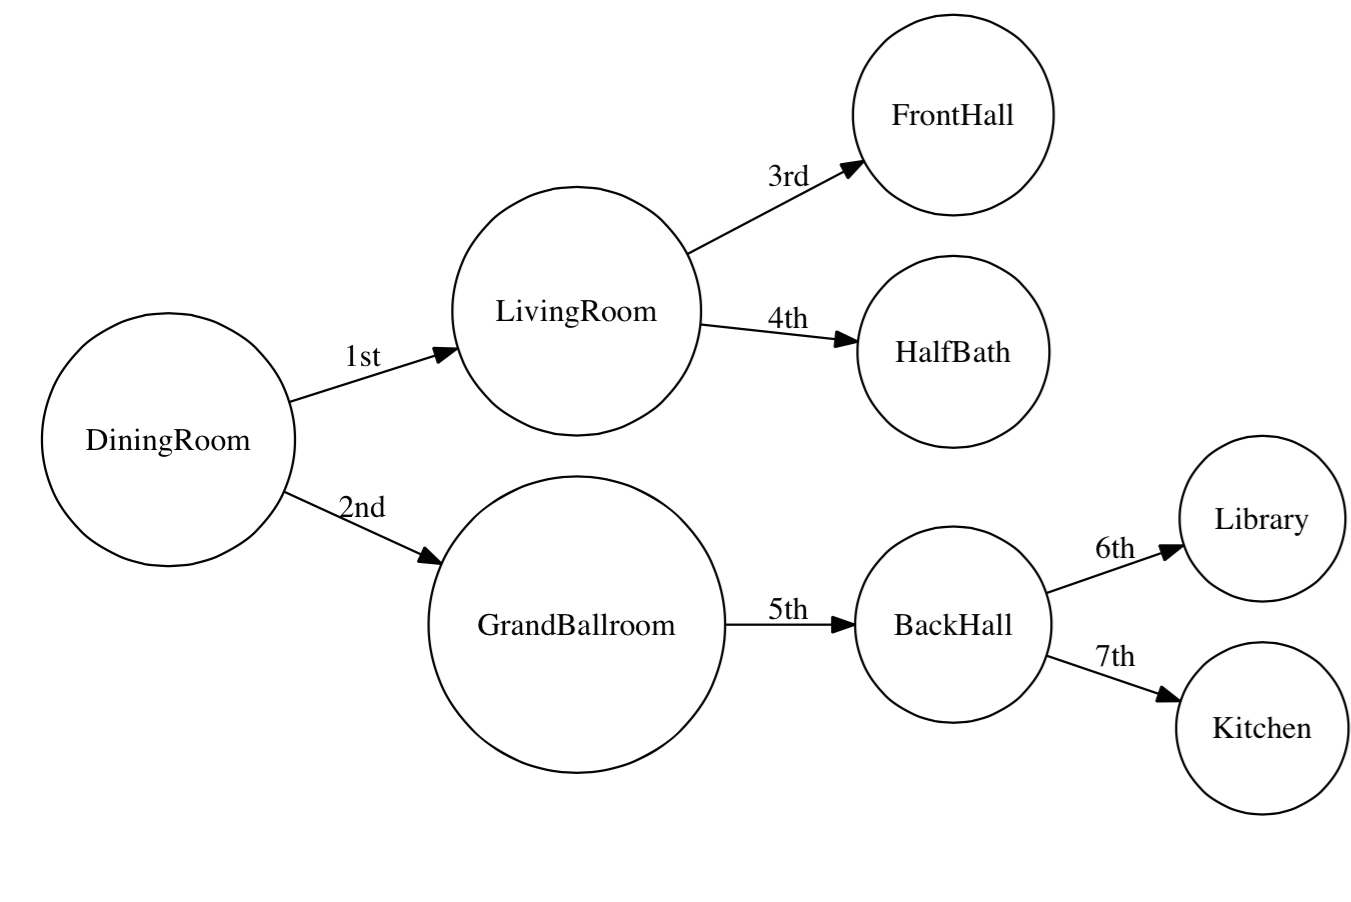
\includegraphics[scale=.5]{./images/BFS.png}

The total cost of the path to the Kitchen is 5. 


\item
Draw a graph of the search tree that will be created if the agent uses the
Uniform Cost Search strategy to solve this problem.  Draw only nodes that will
actually be expanded in the course of the search.

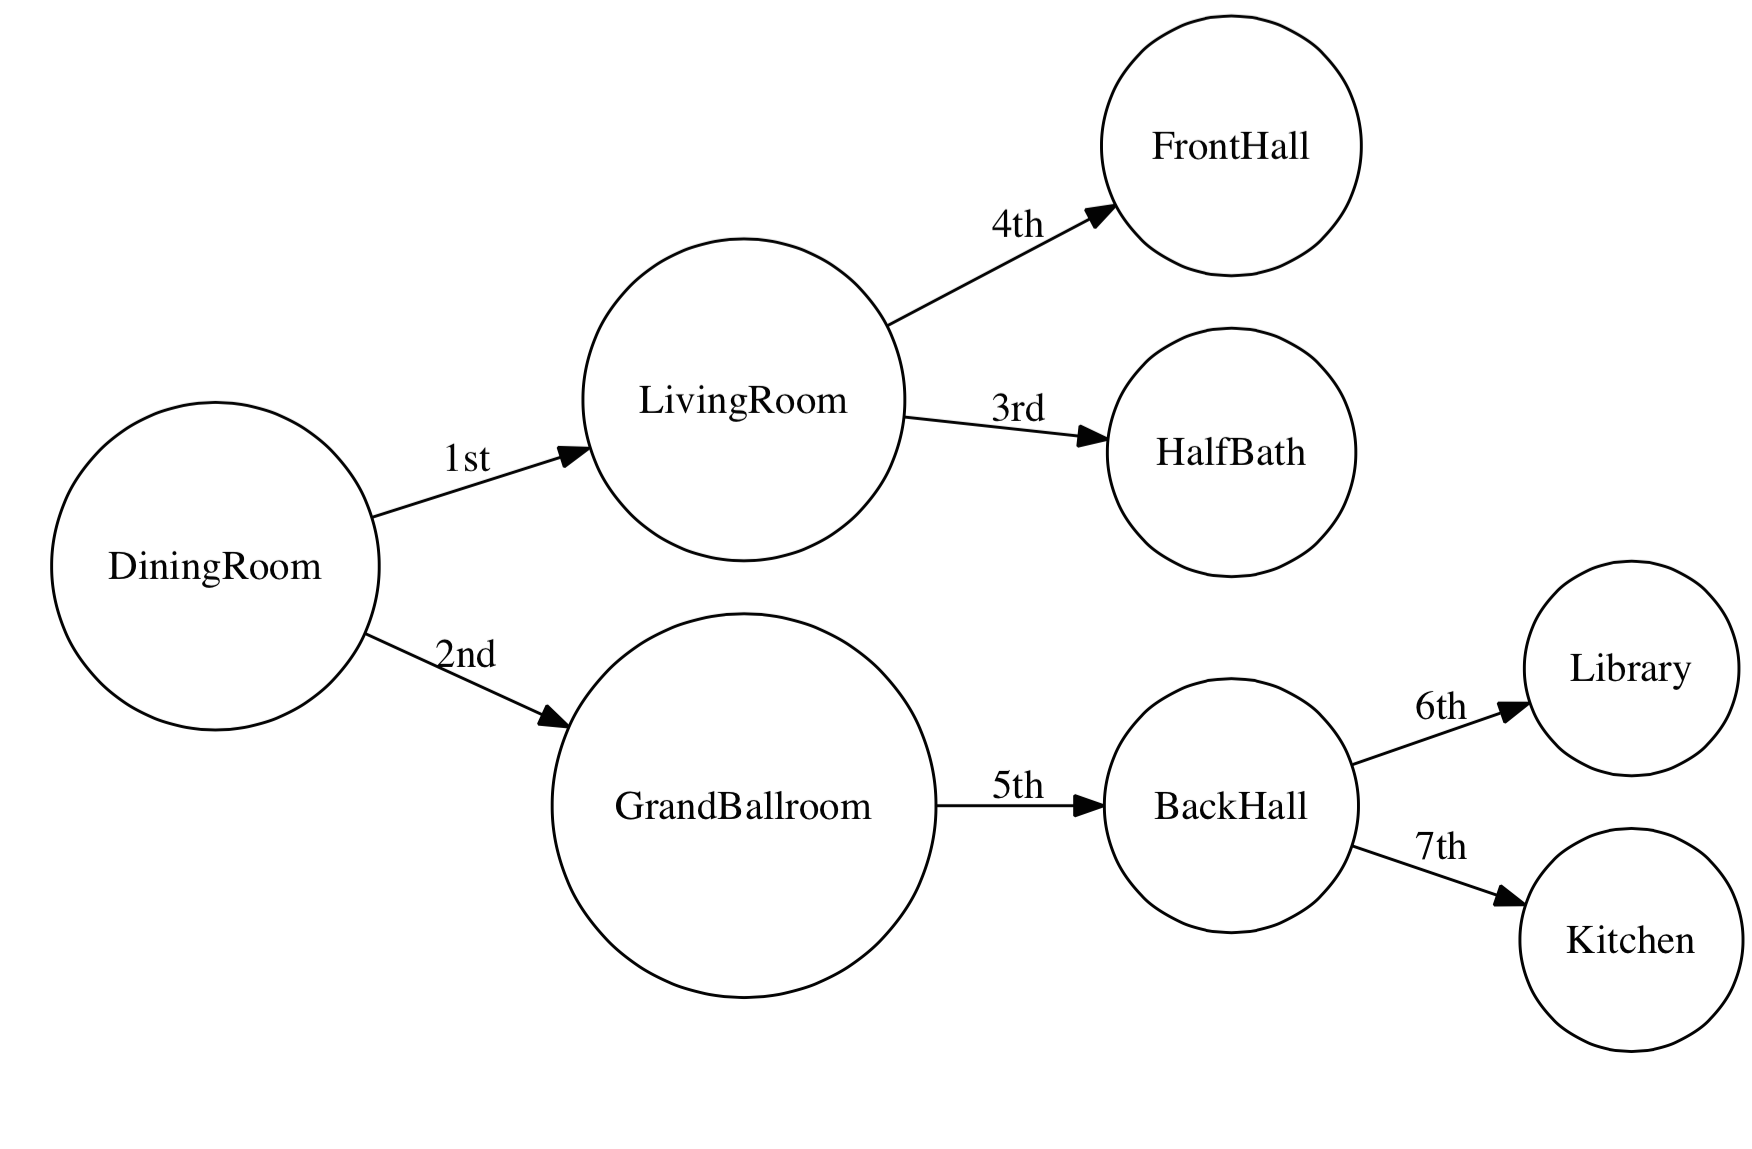
\includegraphics[scale=.4]{./images/UCS.png}

The total cost of the path to the Kitchen is 5. 


\item
With respect to your program implementation, create a table listing the
number of nodes expanded by each search algorithm for each of the gridworld
problems, as well as the approximate runtime (use the \ttt{time} command, and
report \ttt{user} time), and the total cost of the path to the goal that was
found.  Note that timing information is useful only for very rough
relative comparisons, and is not a useful metric for rigorous analysis.  If your
program failed to find a solution, report how it failed.
The table should look something like the following, only with all the maps, and
with the numbers filled in.

\n\noindent
\begin{table}[h]
\begin{tabular}{lllllllllllll}
\textbf{map} & \textbf{BFS} & \textbf{nodes} & \textbf{time} & \textbf{cost} & \textbf{DFS} & \textbf{nodes} & \textbf{time} & \textbf{cost} & \textbf{A*} & \textbf{node} & \textbf{time} & \textbf{cost} \\
map1         &              & 7              & .084          & 7             &              & 7              & .086          & 7             &             & 7             & .087          & 7             \\
map2         &              & 14             & .089          & 14            &              & 14             & .089          & 14            &             & 14            & .094          & 14            \\
map3         &              & 30             & .087          & 14            &              & 24             & .091          & 14            &             & 27            & .094          & 14            \\
map4         &              & 42             & .090          & 22            &              & 27             & .091          & 26            &             & 42            & .096          & 22            \\
map5         &              & 44             & .088          & 15            &              & 24             & .091          & 20            &             & 33            & .096          & 15            \\
map6         &              & 926,824        & 11.838        & 9,499         &              & 37,035         & 10.930        & 37,035        &             & 29,110        & 10.481        & 9,499         \\
map7         &              & 38             & .089          & *             &              & 28             & .086          & *             &             & 38            & .092          & *             \\
map8         &              & 21             & .089          & 21            &              & 13             & .086          & 21            &             & 17            & .090          & 15            \\
map9         &              & 25444          & 0.460         & 357           &              & 581            & .437          & 581           &             & 1523          & .452          & 357          
\end{tabular}
\end{table}


\item Describe the A* heuristic you chose for the gridworld problems.  Justify its
admissibility and discuss its usefulness in solving these problems, in
particular the later ones.

The heuristic I choose is a modified calculation of the manhattan distance. As usual, $f(n) = g(n) + h(n)$ where $g(n)$ is the actual cost to node $n$ from the start. The $h(n)$ is calculated in such a way that it prefers the current node $n$ to be aligned vertically with the $goal$ node. That is, as long as the horizontal distance between $n$ and the goal is more than one, then $f(n) = ManhattanDistance(n, goal)$. Else, $f(n) = g(n)$. The behavior is as follows: in a completely open graph such as map6.txt, the algorithm will move diagonally toward the column the $goal$ node is in. Once there, it will move straight down to the goal just like Dijkstra, expanding very few nodes on this straight line path. This is very very good: only around 29,000 nodes are expanded with this modified manhattan calculation as opposed to about 330,000 nodes expanded if the heuristic is always the true manhattan distance. If a straight line to the $goal$ column cannot be reached (due to blockages), then $h(n)$ will just be the manhattan distance. This is admissable because at no point does $h(n)$ ever exceed the manhattan distance from $n$ to $goal$, thus $h(n)$ never over-estimates the real shortest path to the $goal$. The heuristic is quite useful because it maximizes $h(n)$ subject to the admissability constraint in most cases. For example, $A^*$ expands $\frac{1}{300}$ of the nodes that $BFS$ expands. 

\item Give an example of a problem where BFS would succeed but DFS would fail.
Describe why this example would cause this behavior.

Consider a Graph Search in which the number of states is infinite. The problem could be framed as "find a planet with earth-like qualities in the universe" where states would be defined as unit light-year cubes in 3D space. Assume that this new earth would be a finite distance away from our planet. There is a high probability that depth first search would fail because the universe is infinite (just assume it is) and sparsely populated with matter, so it is easy to get lost in an infinitely deep branch. However, if there exists a planet with earth-like qualities a finite distance away, the breadth at that level is also finite (that level would be comprised of the surface of the 3-sphere with the new earth as a point on the surface and our earth at the center). If the breadth is finite at a level where a goal exists, then BFS will succeed. 

\item Give an example of a problem where DFS would succeed but BFS would fail.
Describe why this example would cause this behavior.

Imagine a single central node as the start. This node has an infinite branching factor - an infinite number of children. Each of these children has infinite children. But the children at this second level are all goal nodes. Thus the graph is fuzzy ball of depth 2 with goal nodes comprising the outside and the start node the center. Then BFS will never finish iterating through the first level and will fail. However, all DFS has to do is travel over two edges and it reaches a goal node, succeeding. 

\item Give an example of a problem where A* will not show improved performance
over BFS.  Describe why this example would cause this behavior.

Assuming the performance measure is directly related to the number of nodes expanded, as we saw earlier, a graph with an unreachable goal is an example of this case. Both BFS and $A^*$ expanded every node in the finite graph before terminating. Another possibility is if there is only one path to the goal, say down a long narrow hallway around which there are no alternatives. 

\item For each of the following heuristics for the gridworld map problems (as
specified in the assignment), state whether the heuristic is admissible, and
then whether it is useful (ie. how good a job does it do of allowing us to
expand as few nodes as possible before finding the goal).  Justify your response. 
\begin{itemize}
  
  \item $h(n)= 2$ for all $n$: This is not admissable. Consider the case when the current node is within distance 2 from the goal node. Then $h(n)$ will overestimate the true distance to the goal, and thus suboptimal behavior can occur. 
  \item $h(n)= 0$ if $n$ is the goal, $1$ otherwise. This is Dijkstra's algorithm, for $h(n) = g(n)$ for all nodes besides the goal. This is guarunteed to find the shortest path, but it's performance is as bad as BFS. Thus this heuristic is useless, yet it is admissable.  
  \item $h(n)= $ Euclidean distance from current node to goal node: This is certainly admissible, since actual distance in our grid worlds is manhattan distance. By triangle inequality theorem, the sum of the lengths of the sides of a traingle are greater than the hypotenuse $(a + b) > (a^2 + b^2)^{1/2}$. The length of the hypotenuse is the euclidian distance from one vertex of the triangle to the other, while the quantity $(a + b)$ is the manhattan distance. Since the hypotenuse can never be longer than the true manhattan distance, the heuristic never overestimates the shortest real distance; thus it is admissable. This heuristic is moderately useful at best. Maximum performance would be achieved if the sides of the triangle
  \item $h(n)= $ Twice the Euclidean distance from current node to goal node: this is not admissable because the triangle inequality $(a + b) > (a^2 + b^2)^{1/2}$ fails in the case where $a = 1, b = 2$ (clearly $2*5^{1/2}$ is greater than 3). Thus there exists a possible goal node position for which $h(n)$ overestimates the shortest path. 
  \item $h(n)= $ Manhattan distance from current node to goal node: this is the optimal heuristic for gridworld problems. It is admissable since the true gridworld path length is always greater than or equal to the manhattan distance (equality holds when a graph contains no obstacles and all nodes have uniform cost. Barring the last two assumptions, true path cost can only increase). Thus, manhattan distance can never overestimate true path cost to goal. Furthermore, this is a heuristic that does a good job maximizing $h(n)$ subject to the admissability constraint. In fact, it is maximized in an unobstructive graph with constant uniform node costs. In other, less-perfect graphs, this is still a very good heuristic. See the results in the table above in which $A^*$ uses a manhattan distance heuristic. Notice how it expands $\frac{1}{300}$ of the nodes that BFS does. 
  \item $h(n)= $ One half the Manhattan distance from current node to goal node: this is  admissable. In a grid world, the true distance to the goal cannot be less than the manhattan distance, and one half that that could only underestimate the true distance. However, this might not be very useful, in fact it could be less useful than the euclidian distance heuristic (consider the right isosceles triangle of side length $a$ where the goal and start nodes are on non-right-angle vertices, the hypotenuse ($\sqrt{2}a$) is greater than the sum of  $\frac{1}{2}a + \frac{1}{2}a$. So this heuristic could be quite useless. 
 
\end{itemize}

\end{questionList}

\end{document}
